\documentclass[12pt, a4paper]{article}

\usepackage[margin=2.5cm]{geometry}
\usepackage{graphicx}
\usepackage{amsmath}
\usepackage{amssymb}
\usepackage{booktabs}
\usepackage{hyperref}
\usepackage{listings}
\usepackage{xcolor}
\usepackage{caption}
\usepackage{subcaption}
\usepackage{parskip}
\usepackage{titlesec}
\usepackage{fancyhdr}

\hypersetup{
    colorlinks=true,
    linkcolor=blue!60!black,
    urlcolor=blue!60!black,
}

\lstset{
    language=Python,
    basicstyle=\ttfamily\small,
    keywordstyle=\color{blue!70!black}\bfseries,
    commentstyle=\color{gray},
    stringstyle=\color{orange!80!black},
    breaklines=true,
    frame=single,
    backgroundcolor=\color{gray!8},
    numbers=left,
    numberstyle=\tiny\color{gray},
    xleftmargin=1.5em,
    framexleftmargin=1.5em,
}

\pagestyle{fancy}
\fancyhf{}
\rhead{Collective Robotics -- Tutorial 2}
\lhead{Gandhi, Machida}
\cfoot{\thepage}

\title{
    \vspace{-1cm}
    \textbf{Collective Robotics -- Tutorial 2}\\[0.3em]
    \large Robot Behaviors and Swarm Systems\\[0.5em]
    \normalsize Hochschule Bonn-Rhein-Sieg\\
    Prof.\ Dr.\ Javad Ghofrani
}
\author{Bhavesh Gandhi \and Jaqueline Machida}
\date{31.05.2026}

\begin{document}

\maketitle
\thispagestyle{fancy}
\tableofcontents
\newpage

% =============================================================================
\section{Task 1 -- Behaviors of a Single Robot}
% =============================================================================

\subsection{Overview}

We implemented three reactive behaviors for a simulated vacuum-cleaner robot in
the TurtleBot3 House world: \textbf{collision avoidance}, \textbf{wall
following}, and \textbf{vacuum-cleaner coverage} (boustrophedon).  The robot
model, world, launch files, and ROS\,2 nodes all live in the
\texttt{single\_robot} package under \texttt{Task~1/ros2\_ws/}.

\paragraph{Simulation setup.}
We used \textbf{ROS\,2 Jazzy} with \textbf{Gazebo Harmonic}.  A custom SDF model
(\texttt{models/vacuum\_cleaner/model.sdf}) defines a cylindrical robot
(radius~0.17~m, height~0.09~m) with two differential-drive wheels, a passive
caster, and a 360° 2D lidar mounted on top.  The Gazebo
\texttt{DiffDrive} system provides the wheel control, and a
\texttt{ros\_gz\_bridge} parameter bridge translates \texttt{/scan},
\texttt{/cmd\_vel}, \texttt{/odom}, \texttt{/tf}, and \texttt{/joint\_states}
between Gazebo and ROS\,2.

A snapshot of the simulation environment (TurtleBot3 House) with the vacuum
cleaner robot spawned inside it is shown in Figure~\ref{fig:task1-screenshot}.

\begin{figure}[h]
    \centering
    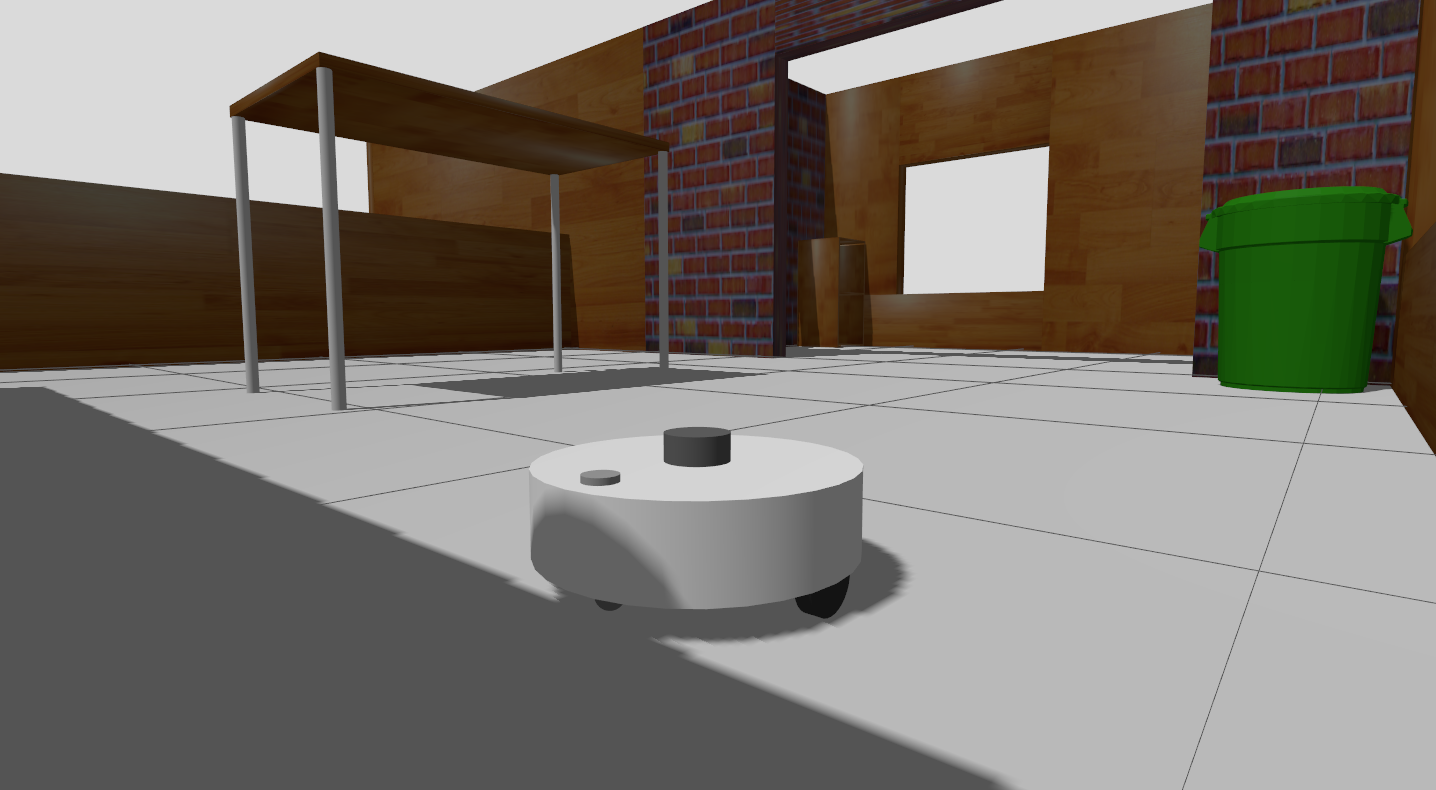
\includegraphics[width=0.85\textwidth]{Task 1/ros2_ws/results/screenshot.png}
    \caption{Top-down view of the vacuum-cleaner robot in the TurtleBot3 House
             world used for all three Task~1 experiments.}
    \label{fig:task1-screenshot}
\end{figure}

\paragraph{Common design.}
All three behaviors share the same skeleton: a \texttt{LaserScan} subscriber
caches the latest scan, a timer drives a 20~Hz control loop that walks the
scan once per tick to compute sector minima (front cone of $\pm30°$, plus
left/right halves), updates a finite state machine, and publishes a
\texttt{Twist} on \texttt{/cmd\_vel}.

\subsection{Collision Avoidance}

The robot drives forward at constant speed and rotates in place when an
obstacle enters the front cone.  The FSM has two states:

\begin{itemize}
    \item \textbf{CRUISE} -- publish \texttt{linear.x = CRUISE\_SPEED}.
    \item \textbf{AVOID} -- stop linear, rotate at $\pm$\texttt{TURN\_SPEED}
          toward the freer side (chosen at transition time by comparing
          left/right sector minima).
\end{itemize}

\textbf{Hysteresis} on the trigger and clear distances
(\texttt{TRIGGER\_DISTANCE = 0.35~m}, \texttt{CLEAR\_DISTANCE = 0.55~m})
prevents the robot from chattering between the two states near the threshold.
The turn direction is frozen for the duration of an AVOID episode so the robot
commits to one direction rather than oscillating between left and right.

A demonstration video is available at
\url{https://youtu.be/UbriNbjf1nM}.

\subsection{Wall Following}

The robot performs right-wall following using a small FSM and a PD controller
on the side-cone distance:

\begin{itemize}
    \item \textbf{FIND\_WALL} -- drive forward until the right-side cone (a
          $\pm30°$ window centered at $-\pi/2$) sees a wall within
          \texttt{WALL\_DETECT\_DISTANCE = 0.8~m}.
    \item \textbf{FOLLOW} -- maintain a target distance of $0.4~$m to the right
          wall using $\omega = K_P \cdot e + K_D \cdot \dot e$, where
          $e = d_{\mathrm{target}} - d_{\mathrm{right}}$.  Positive error
          (too close) commands a left turn (away from the wall); negative
          error (too far) commands a right turn (toward the wall).
    \item \textbf{CORNER\_TURN} -- when the front cone is blocked (concave
          corner), stop linear and rotate left in place until the front
          clears.  Hysteresis on \texttt{CORNER\_TRIGGER}/\texttt{CORNER\_CLEAR}
          prevents flapping.
\end{itemize}

Convex corners are handled implicitly: when the right wall disappears, the
measurement is clamped to \texttt{WALL\_DETECT\_DISTANCE}, which gives a
constant rightward bias that curls the robot back toward the wall.  An edge
case handled during development was the initial transition: entering FOLLOW
from a \emph{front} detection (instead of a side detection) gave the PD
controller no usable measurement and caused the robot to spin in place; the
fix was to require the wall to appear on the right side before entering
FOLLOW, and to redirect head-on detections directly to CORNER\_TURN.

A demonstration video is available at
\url{https://youtu.be/crJzeYGZqmE}.

\subsection{Vacuum-Cleaner Coverage}

\paragraph{Coverage strategies.}
Before settling on an implementation we considered three families of strategies
for a vacuum-cleaning robot:

\begin{enumerate}
    \item \textbf{Random walk.}  Drive straight; on collision, turn by a random
          angle and continue.  The simplest possible strategy, requiring no
          state beyond the FSM and no odometry.  Given enough time it
          probabilistically covers the entire reachable area, but the time to
          near-full coverage is long and the trajectory looks erratic.

    \item \textbf{Lawnmower (boustrophedon).}  Drive forward until a wall,
          U-turn while shifting laterally by one body width, then drive in
          the opposite direction.  The repeating parallel stripes cover the
          area systematically and quickly.  The main challenges are
          (i) executing crisp $90°$ turns so successive stripes remain
          parallel to each other and perpendicular to the walls, and
          (ii) handling the room boundary: once the robot has marched all the
          way across the room, the lateral shift gets blocked by the parallel
          wall and the robot becomes stuck oscillating in the last stripe.
          Reversing the shift direction at that point keeps the robot moving
          but only re-covers area it has already cleaned, and it does not
          guarantee that gaps left by inaccurate stripe spacing get filled.

    \item \textbf{Map-based planning.}  Build an occupancy map of the
          environment, track the robot's pose against it, and direct the
          robot toward un-cleaned cells while restarting the local
          boustrophedon sweep there.  This is what current commercial vacuum
          robots do.  It dominates the other two in efficiency and coverage
          guarantee, but requires SLAM and a planning layer.
\end{enumerate}

\paragraph{Our implementation.}
We implemented the boustrophedon strategy, since it directly demonstrates the
characteristic ``zig-zag'' coverage pattern.  The FSM has four states:

\begin{itemize}
    \item \textbf{SWEEP} -- drive forward at \texttt{FORWARD\_SPEED} until the
          front cone reads below \newline \texttt{TRIGGER\_DISTANCE}.
    \item \textbf{TURN\_A} -- rotate $90°$ in the current
          \texttt{turn\_direction}, using odometry yaw as the target.
    \item \textbf{SHIFT} -- drive forward by one \texttt{BODY\_WIDTH} (0.34~m)
          measured against \texttt{/odom} position, or until the front cone
          trips, or until a wall-clock timeout fires.
    \item \textbf{TURN\_B} -- rotate another $90°$ in the same direction,
          which inverts the heading and leaves the robot laterally shifted by
          one stripe.  The \texttt{turn\_direction} is then flipped so the
          next U-turn rotates the other way, keeping the lateral shift on the
          same side of the room and producing parallel stripes.
\end{itemize}

\paragraph{Turn precision (proportional control).}
A bang-bang turn at full \texttt{TURN\_SPEED} produces a large yaw overshoot
when commanded to stop, because the diff-drive plugin has finite angular
deceleration.  After a single U-turn the heading was off by ${\sim}20°$, and
this drift accumulated each cycle until the ``parallel stripes'' became visibly
non-parallel.  We replaced the bang-bang turn with a proportional controller,
$\omega = \mathrm{clamp}(K_P \cdot \mathrm{yaw\_err},\,\pm \texttt{TURN\_SPEED})$:
the command runs at maximum speed far from the target and ramps smoothly to
zero near it, so the angular velocity is already small when the state
transitions out and the overshoot becomes negligible.  The same trick on the
SHIFT distance produces clean stripe spacing.

\paragraph{Stuck handling.}
The original SHIFT exit conditions (full body width covered or front cone
tripped) did not catch all stuck situations. We added a wall-clock
timeout on SHIFT: if \texttt{BODY\_WIDTH} has not been covered within
\texttt{SHIFT\_TIMEOUT} seconds, the SHIFT exits anyway and the U-turn
completes.

\paragraph{Limitations.}
As discussed above, the boustrophedon strategy does not detect when the
parallel wall on the opposite side of the room has been reached, so the robot
keeps zig-zagging in the last stripe until it is stopped manually.  A natural
extension would be to detect that several consecutive SHIFT phases failed to
make significant progress and either declare coverage complete (stop), reverse
the lateral direction to march back, or hand off to a map-based planner.

A demonstration video is available at
\url{https://youtu.be/eYblzjBrKoo}.

\newpage
% =============================================================================
\section{Task 2 -- Behaviors of Robot Swarms}
% =============================================================================

\subsection{Overview}

We implemented and analyzed a decentralized \textbf{swarm aggregation}
behavior using the \textbf{ARGoS\,3} simulator and a two-state \textbf{Lua}
controller.  A swarm of \texttt{foot-bot} robots operates in a closed
$4~\text{m} \times 4~\text{m}$ arena.  By following a simple local rule -- stop
and wait whenever a neighbor is detected -- a single stable cluster emerges as
a global property of the swarm.  We analyzed how the speed and stability of
cluster formation depend on swarm size for
$N \in \{5, 10, 20, 30, 50\}$.  The full source, configuration, and analysis
scripts live under \texttt{Task~2/}.

\subsection{Implementation}

\paragraph{Two-state FSM (\texttt{task2.lua}).}
Each robot runs the same decentralized controller with two states:

\begin{itemize}
    \item \textbf{WANDER} -- drive forward at \texttt{MAX\_VELOCITY = 20~cm/s},
          steering away from walls and other robots using the 24 infrared
          proximity sensors.  At every step, query the Range-and-Bearing (RAB)
          sensor; if any other robot is detected within
          \texttt{STOP\_DISTANCE = 25~cm}, transition to \textbf{STOPPED} and
          initialize a wait timer.  LED indicator: green.
    \item \textbf{STOPPED} -- set wheel velocities to $(0, 0)$ and decrement
          the \texttt{WAIT\_TICKS = 30} (\,$=3.0$~s) timer.  When the timer
          reaches zero, return to \textbf{WANDER}.  LED indicator: red.
\end{itemize}

\paragraph{Obstacle avoidance.}
Avoidance is computed as a virtual repulsion vector summed over the 24
proximity readings:
\[
    \mathbf{F}_{\text{repulsion}} = -\sum_{i=1}^{24}
        \bigl(v_i \cos\alpha_i\,\mathbf{\hat x} +
              v_i \sin\alpha_i\,\mathbf{\hat y}\bigr),
\]
where $v_i \in [0, 1]$ is the proximity reading and $\alpha_i$ is the sensor
angle.  When $\|\mathbf{F}_{\text{repulsion}}\| < 0.05$ the robot drives
straight; otherwise the differential wheel speeds are adjusted toward the
direction of $\mathbf{F}_{\text{repulsion}}$ using \texttt{TURN\_GAIN = 2.0},
clamped to $[-20, 20]~\text{cm/s}$.

\paragraph{Experiment pipeline.}
\texttt{task2.argos} defines the arena, the swarm population, sensors, and
loop functions that log the per-tick fraction of stopped robots and per-robot
neighbor counts to CSV.  \texttt{run\_experiments.py} patches the swarm size
in a temporary copy of the configuration, runs \texttt{argos3} headlessly
(\texttt{-z}) for $300~$s at $10$~ticks/s for each $N \in \{5, 10, 20, 30,
50\}$, and emits per-run and aggregated CSVs under \texttt{data/}.
\texttt{plot\_results.py} consumes the dataset and writes the three figures
discussed below.

A cluster is defined as successfully formed when \textbf{99\,\% of the swarm}
is simultaneously in the \texttt{STOPPED} state.

\subsection{Subtask a -- Stop on Neighbor Detection \& Subtask b -- Bounded Wait Time}

Both subtasks are realized by the FSM above.  The local rule (``stop on
neighbor detection'') corresponds to the \texttt{WANDER}~$\to$~\texttt{STOPPED}
transition triggered by the RAB sensor at $25~$cm.  The bounded wait time is
the $3.0$~s timer attached to the \texttt{STOPPED} state, after which the
robot resumes wandering.

\subsection{Subtask c -- Tuning for Aggregation: Cluster Kinetics}

Figure~\ref{fig:task2-stopped} shows the fraction of stopped robots over time
for the five swarm sizes.

\begin{figure}[h]
    \centering
    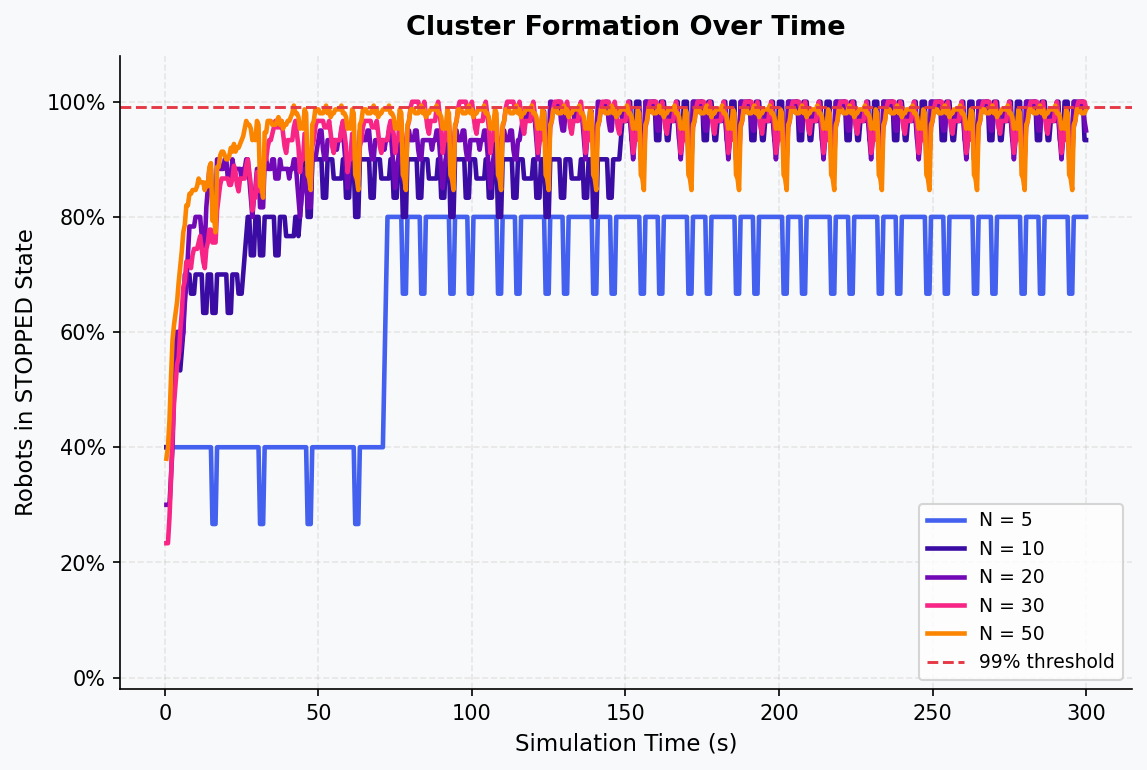
\includegraphics[width=0.85\textwidth]{Task 2/plots/task2_stopped_over_time.png}
    \caption{Fraction of stopped robots over time for each swarm size.
             A cluster is declared formed when the curve reaches~99\,\%.}
    \label{fig:task2-stopped}
\end{figure}

\paragraph{Observations.}
\begin{itemize}
    \item \textbf{$N = 50$ (dense):} extremely rapid aggregation; the stopped
          fraction rises sharply and stabilizes at 100\,\% within $\sim 50$~s.
    \item \textbf{$N = 30,\,20,\,10$ (medium):} steady, reliable aggregation,
          reaching the 99\,\% threshold progressively later but remaining
          stable thereafter.
    \item \textbf{$N = 5$ (sparse):} fails to aggregate -- the stopped
          fraction oscillates randomly and never reaches 99\,\%.  Encounter
          rates are too low to sustain a growing cluster in this arena size.
\end{itemize}

\subsection{Subtask d -- Effect of Swarm Size on Speed and Stability}

\paragraph{Time to cluster.}
Figure~\ref{fig:task2-ttc} and Table~\ref{tab:task2-ttc} summarize the time
required for the swarm to reach the 99\,\% threshold.

\begin{figure}[h]
    \centering
    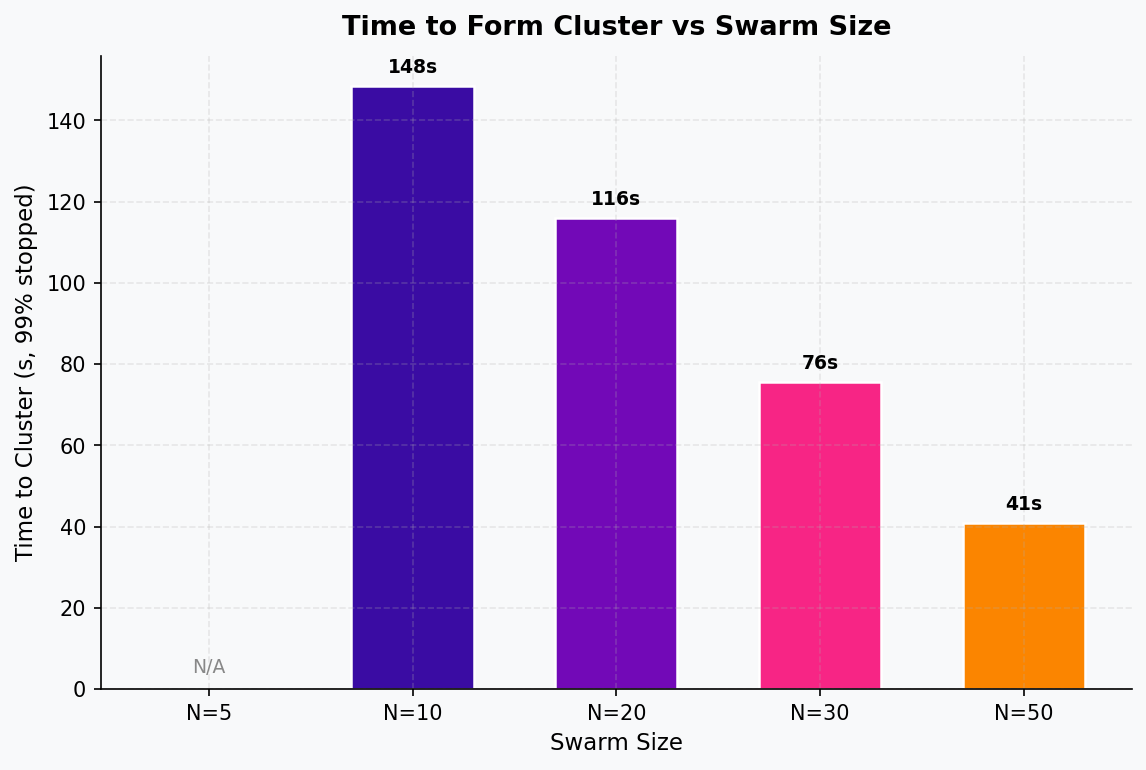
\includegraphics[width=0.7\textwidth]{Task 2/plots/task2_time_to_cluster.png}
    \caption{Time to form a cluster (99\,\% stopped) vs.\ swarm size.}
    \label{fig:task2-ttc}
\end{figure}

\begin{table}[h]
\centering
\begin{tabular}{lc}
\toprule
\textbf{Swarm size $N$} & \textbf{Time to cluster (s)} \\
\midrule
$5$  & did not cluster \\
$10$ & $148.5$ \\
$20$ & $116.0$ \\
$30$ & $75.5$  \\
$50$ & $41.0$  \\
\bottomrule
\end{tabular}
\caption{Time required for the stopped fraction to reach 99\,\%.}
\label{tab:task2-ttc}
\end{table}

The relationship is markedly non-linear: increasing $N$ reduces the time to
cluster super-linearly.  Because the arena is fixed, a larger $N$ corresponds
directly to higher density, which raises the encounter rate.  Once a few
robots have stopped, they act as ``nucleation sites'' that wandering robots
collide with, stop next to, and so grow the cluster -- a positive-feedback
loop that runs much faster at high density.

\paragraph{Cluster stability.}
Figure~\ref{fig:task2-stab} and Table~\ref{tab:task2-stab} report the
distribution of per-robot neighbor counts in the last $3.0$~s of each run.

\begin{figure}[h]
    \centering
    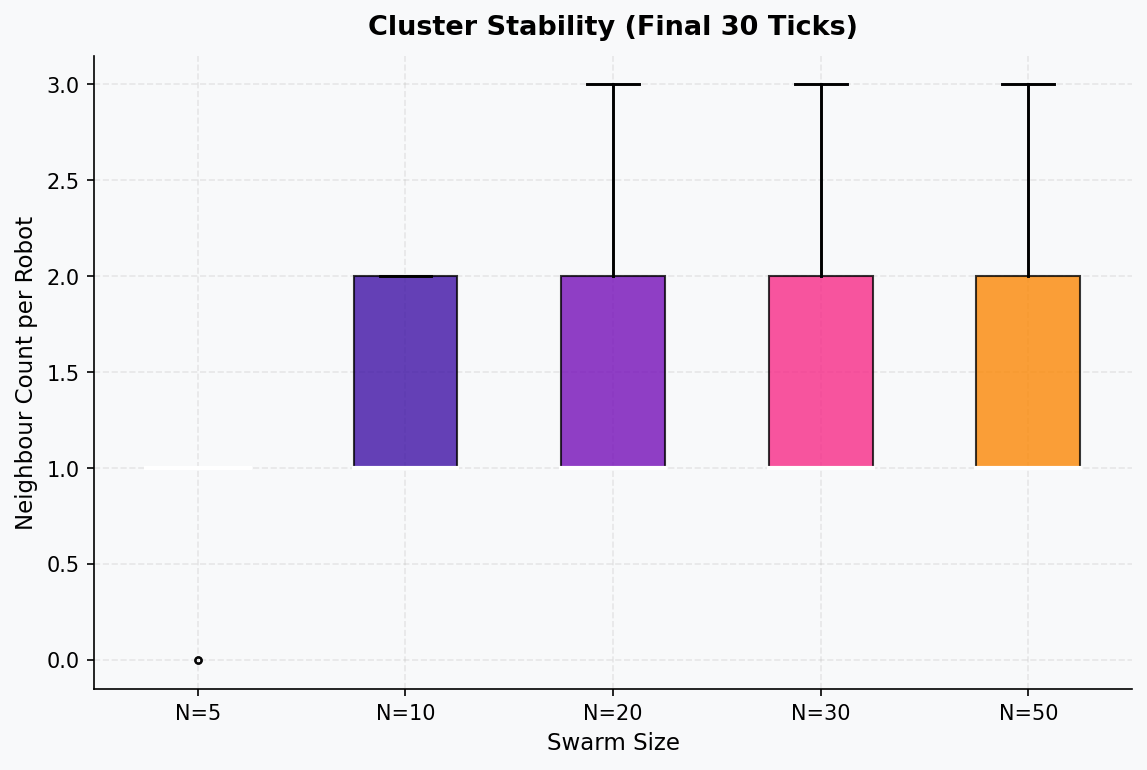
\includegraphics[width=0.7\textwidth]{Task 2/plots/task2_cluster_stability.png}
    \caption{Distribution of neighbor counts per robot in the final 30 ticks
             of the simulation.}
    \label{fig:task2-stab}
\end{figure}

\begin{table}[h]
\centering
\begin{tabular}{lcccc}
\toprule
\textbf{$N$} & \textbf{Mean} & \textbf{Median} & \textbf{Min} & \textbf{Max} \\
\midrule
$5$  & $0.80$ & $1$ & $0$ & $1$ \\
$10$ & $1.40$ & $1$ & $1$ & $2$ \\
$20$ & $1.40$ & $1$ & $1$ & $3$ \\
$30$ & $1.40$ & $1$ & $1$ & $3$ \\
$50$ & $1.44$ & $1$ & $1$ & $3$ \\
\bottomrule
\end{tabular}
\caption{Final-window neighbor-count statistics per swarm size.}
\label{tab:task2-stab}
\end{table}

For all successful runs ($N \geq 10$), the median neighbor count is $1$ with
a tight $[1, 3]$ spread, indicating a stable, tight aggregate.  For $N = 5$
the minimum drops to $0$: robots frequently drift apart faster than new
neighbors arrive to reinforce the stopping behavior, and the cluster
dissolves.

\subsection{Discussion}

The system illustrates how a complex global structure (a single cluster)
arises from a simple, local rule (``stop for a few seconds if anyone is
nearby'') with no central control, no global localization, and no
communication beyond proximity detection.  The mechanism is positive
feedback: stopped robots act as physical obstacles that other robots steer
toward and then stop next to themselves.

A critical density threshold ($N \geq 10$ in this arena) is needed for the
positive-feedback loop to outrun the bounded wait time -- below it, stopped
robots time out and resume wandering before new neighbors arrive, and no
cluster forms.  Above the threshold, the time to cluster scales
super-linearly with swarm size.

\newpage
% =============================================================================
\section{Completed Tasks}
% =============================================================================

\begin{center}
\begin{tabular}{lll}
\toprule
\textbf{Task} & \textbf{Description} & \textbf{Status} \\
\midrule
1 & Collision avoidance behavior (FSM, ROS\,2 + Gazebo)        & \checkmark \\
1 & Wall follower (PD + corner FSM, ROS\,2 + Gazebo)           & \checkmark \\
1 & Vacuum cleaner (boustrophedon coverage, ROS\,2 + Gazebo)   & \checkmark \\
\midrule
2 & Stop on neighbor detection (ARGoS, Lua FSM)                & \checkmark \\
2 & Bounded wait time before resuming wander                   & \checkmark \\
2 & Parameter tuning to obtain a single aggregated cluster     & \checkmark \\
2 & Analysis of swarm size vs.\ speed and stability of cluster & \checkmark \\
\bottomrule
\end{tabular}
\end{center}

\end{document}
